\section{Docker}

Docker je otevřená platforma pro vývoj, dodání a spouštění aplikací. Umožnuje oddělení aplikací od infrastruktury, tedy můžeme dodávat software rychleji a bez problémů, které se váží k různorodosti prostředí, ve kterém aplikace běží. Svou fylozofií jsou velice podobné virtualním počítačům. Rozdíly mezi těmito různými pohledy na věc budou rozebrány dále v textu. 

Docker zprostředkovává platformu pro zabalení aplikace i se všemi jejímy závislostmi. Izoluje danou aplikaci od ostatních běžících procesů na daném počítači a zajišťuje tak její bezpečí. Docker kontejner je velice nenáročný na hardware, můžeme jich tedy na daném počítači spustit velice mnoho.  

Fylosofie kontejnerů je taková, že každý kontejner je odpovědný pouze za jednu danou část aplikace. Pro příklad máme naší webovou aplikaci. Budeme tedy mít alespoň tři docker kontejnery. Jeden na kterém poběží NGINX a bude zprostředkovávat naší aplikaci uživatelům. Další bude mít naší aplikaci a ve třetím poběží databáze. 

Konterjnery fungují tedy jako malé počítače, mají izolované veškeré svoje systémové zdroje ( paměť, procesy, internetové rozhraní ). Díky tomuto mohou být rychle a jednoduše přidány, nebo odebrány.  


\subsection{Konterjner vs. virtuální počítač}

Virtualizace je odpověď na problém různorodých prostředí mezi vývojáři a zákazníky. Problém ,který virtualizace a kontejnerizace především řeší je různorodost prostředí mezi zákazníkem a dodavatelem softwaru. Při jeho předávání dochází ke změně prostředí, jsou nainstalované jiné verze závislostí a operačního systému a aplikace se může chovat neočekávaně. 

Podíváme se jak se tyto dvě technologie liší a proč se svět žene právě směrem kontejnerizace, když zde již je řešení.

Virtuální počítač je regulérní stroj, který běží na daném hostovi. Tento stroj má svůj kernel, svůj operační systém a ke zdrojům přistupuje přes tzv. hypervizor např.: QEMU, nebo VirtualBox. Hypervizor zprostředkovává přístup virtuálního stroje k systémovým zdrojům. 

Pro to, aby na hostovi, nebo-li na systému, který má nainstalovaný hypervizor mohlo běžet více virtuálních strojů stačí jedna jeho instance. Nevýhoda tohoto řešení je taková, že se mnoho zdrojů duplikuje. Řekněme, že na hostitelském systému poběží tři aplikace. Každá taková aplikace bude izolovaná od ostatních pomocí virtuálního stroje. Dejme tomu, že to bude databáze, webový server a stroj pro vzdáleného uživatele. Níže uvidíme nákres tohoto řešení. 

% https://www.docker.com/resources/what-container
\begin{figure}[!ht]
	\centering
	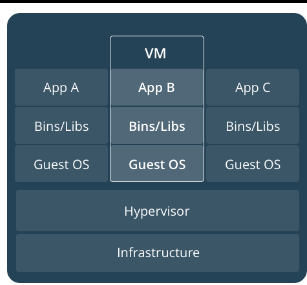
\includegraphics[width=0.73\textwidth, angle=0]{docker-VM.png}
	\caption[Docker VM]{Oddělení aplikací za pomoci hypervizoru a virtuálních strojů.}
	\label{fig:docker-vm}
\end{figure}

To samé, jako je na obrázku výše se pokusíme realizovat pomocí Dockeru a kontejnerů. Kontejnery, jelikož využívají overlayFS jsou schopny poskytnout jádro operačního systému kontejneru bez zbytečné kopie a využívají copy-on-write funkcionality. Níže uvidíme jak za pomoci jmenných prostorů, kontrolních skupin a overlayFS je tento přístup úspornější a rychlejší než virtualizace. 


\begin{figure}[!ht]
	\centering
	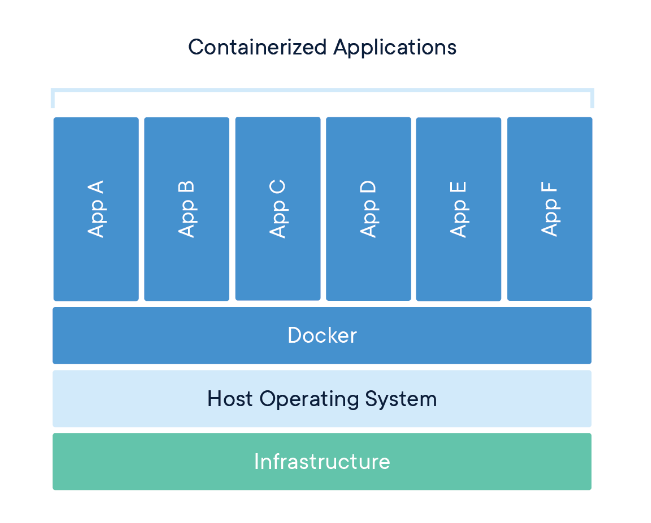
\includegraphics[width=0.8\textwidth, angle=0]{docker-docker.png}
	\caption[Docker kontejnery]{Oddělení aplikací za pomoci Dockeru}
	\label{fig:docker-docker}
\end{figure}

Místo, které jsme na hostitelském systému ušetřili však není jediná výhoda. Na tomto příkladu se však rozdíly mezi těmito technologiemi vysvětlují nejlépe. Dalšími výhodami je rychlost spuštění kontejneru a virtuálního stroje. Při spuštění se pouze připojí obraz OS, vytvoří se izolované procesy a popřípadě se omezí i zdroje, které má kontejner využívat. Nehledě na to, že pokud kontejner nemá omezení nebo limit využitých zdrojů alokuje si je dynamicky oproti virtuálnímu počítači, který si pro sebe naalokuje danou paměť při spuštění.  


\subsection{Stavební kameny Dockeru}

Jak je již uvedeno v předešlé kapitole, Docker využívá vychytávky linuxového kernelu pro svojí funkcionalitu. Díky tomuto perfektně funguje na počítačích, kde běží OS založený na Linuxu. V následujících sekcích budou tyto technologie blíže popsány a bude vysvětlena jejich důležitost. 


\begin{figure}[!ht]
	\centering
	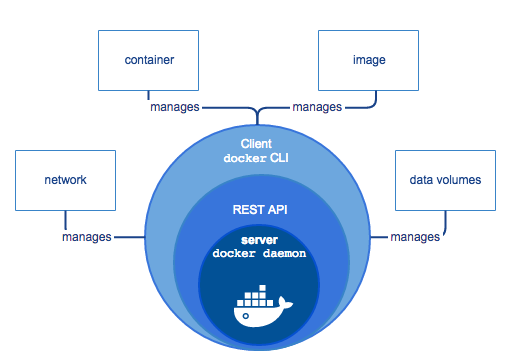
\includegraphics[width=0.8\textwidth, angle=0]{docker-architecture.png}
	\caption[Docker architektura]{Docker a jeho komponenty.}
	\label{fig:docker-architecture}
\end{figure}

%TODO Jak jsou na tom jiné OS

\subsubsection{Jmenné prostory}

Jmenné prostory zastřešují veškeré zdroje systému tak, že každý proces spuštěn v daném prostoru může používat pouze prostředky, které se váží k tomuto prostoru. Každému procesu se to jeví tak, že má svoje vlastní globální prostředky, které mohou vidět i ostatní procesy z jmenného prostoru, ale ne z jiného. V tabulce \ref{tab:Jmenne prostory} je možné videt, jaké jmenné prostory lze v Linuxu nalézt.

% parametry pro table: h! = nejblize
% p{5cm} na zalomovani bunky
\begin{table}[!ht]
  \begin{center}
	\caption{Linuxové jmenné prostory}
    \label{tab:Jmenne prostory}
    \begin{tabular}{|l|l|} 
    	  \hline
      \textbf{Jméno} & \textbf{Popis} \\
      \hline

	  Cgroup  &  Cgroup root adresář\\
	  IPC     &  Systém pro komunikaci procesů, POSIX fronty\\
	  Network &  Síťové rozhraní, protocoly, porty, etc\\
      Mount   &  Připojená zařízení\\
      PID     &  ID procesů\\
      User    &  Uživatelská ID a ID skupin\\
      UTS     &  Hostname a NIS doménu\\   
      
      \hline
    \end{tabular}
  \end{center}
\end{table}

Při spuštění kontejneru dojde k vytvoření procesu na hostitelském systému. Procesy dostanou od systému nějaké PID a chovají se jako normální procesy. Pokud se však přihlásíme do kontejneru (command: docker exec -it name bash) a podíváme se na procesy běžící v daném kontejneru uvidíme, že procesy mají jiná PID a určitě mají i PID=1. Toto nám umožňují jmenné prostory.

Každý kontejner může mít svůj vlastní souborový systém a svoje síťové rozhraní. Vše co můžeme oddělit mezi hostitelem a kontejnery je uvedeno v tabulce výše. 

\subsubsection{Kontrolní skupina}

Je to vlastnost Linuxového kernelu. Jejich hlavní funkcí je limitovat zdroje. V Dockeru se používají protože dovolují sdílet prostředky mezi hostitelským systémem a dalšímy kontejnery. 

Často dochází k záměně pojmů mezi kontrolními skupinami a jmennými prostory. Znovu to tedy shrňme. Kontrolní skupinz, nebo-li cgroups omezují co můžeme použít a jemenné prostorz nebo-li namespaces omezují co jsme schopni vidět v systému. 

\subsubsection{Docker daemon}

Docker daemon nebo-li dockerd poslouchá dotazy na docker API a spravuje objekty jakou jsou docker obrazy, kontejnery, síť a úložiště. Komunikuje ale i s dalšími daemony, aby byl schopen řídit službu Docker.

\subsubsection{Docker klient}

Je to primární cesta, jak komunikovat s Dockerem. Když použijeme příkazy, jako jsou "docker run", klient odešle příkazy daemono zmíněného výše. 

\subsubsection{Docker registr}

Docker registr je úložiště pro naše Docker obrazy. Bez předchozího nastavení hledá dockerd obrazy, které chceme spustit ve veřejném Docker registru. Obrazy však mohou být dostupné i lokálně, nebo na nějaké jiné službě, např.: gitlab container registry. 

Do styku s registrem přícházíme hlavně ve chvílích, kdy provádíme příkazý docker pull, docker push a docker run. Tyto příkazy vždy potřebují znát obraz, který bude spouštěn jako základní vrstva pro nový kontejner, nebo bude stáhnut na lokání počítač, či nasdílen do registru.

\subsubsection{Obrazy}

Můžeme si to představit jako šablonu, na které je spuštěn kontejner. Obraz může být složen z vícero obrazů, nebo z nich vycházet. 

Pro vytvoření obrazu je třeba soubor Dockerfile. Tento soubor obsahuje jednoduché kroky, které je třeba vykonat pro vytvoření konkrétního obrazu. Např.: jaké použijeme a zveřejníme porty, jaké balíčky chceme ve vytvořeném obrazu mít atd. 

Každý příkaz v Dockerfilu vytvoří na locálním počítači tzv. vrstvu, kterou při úpravě Dockerfilu mění nebo předělává pouze pokud byla změněna. 

%TODO picture of docker architecture

\subsection{Systémová kontejnery}

Docker kontejnery nejsou však jediné, které se v produkčním prostředí používají. Patří do tzv. aplikačních kontejnerů. Jejich účel je zpravidla spouštět pouze jeden proces. K takovýmto kontejnerům můžeme ještě přidat kontejnerz Rocket. Hlavním rozdílem je to, že rtk nemá na systému spuštěného daemona jako má např. Docker. Při spuštění se tedy pod běžícím spustí další. 

\begin{figure}[!ht]
	\centering
	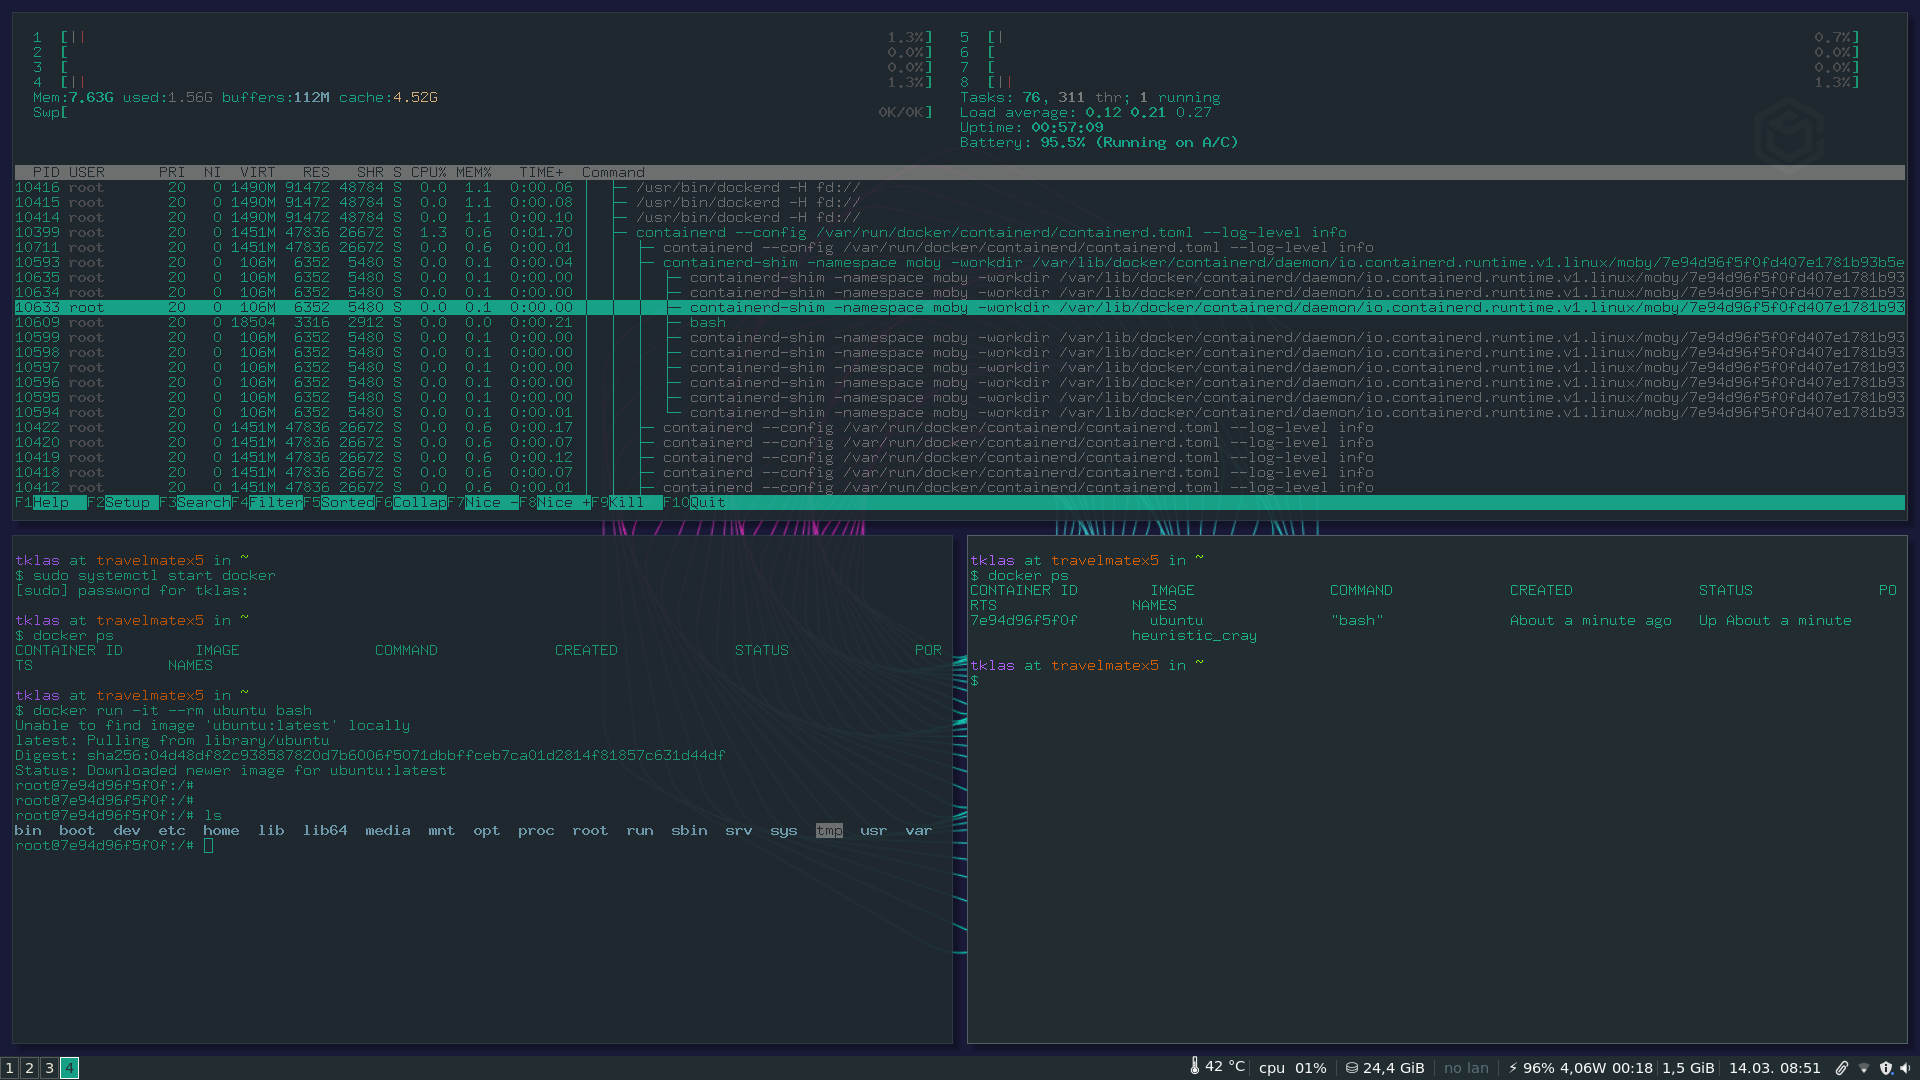
\includegraphics[width=0.95\textwidth, angle=0]{docker-screen.png}
	\caption[Docker kontejnery]{Docker a jeho procesy.}
	\label{fig:docker-list}
\end{figure}

Dále tady máme systémové kontejnery. Ty jsou používané jako klasické OS. Na jednom silném stroji může běžet několik takových kontejnerů a ty mohou uživateli poskytovat oddělené prostředí od celého serveru a nabídnout mu izolovaný prostor od ostattních pomocí výše zmíněných technologií. Tuto možnost zastřešuje projekt LXC později LXD.

%TODO add image of the lxc list

\begin{figure}[!ht]
	\centering
	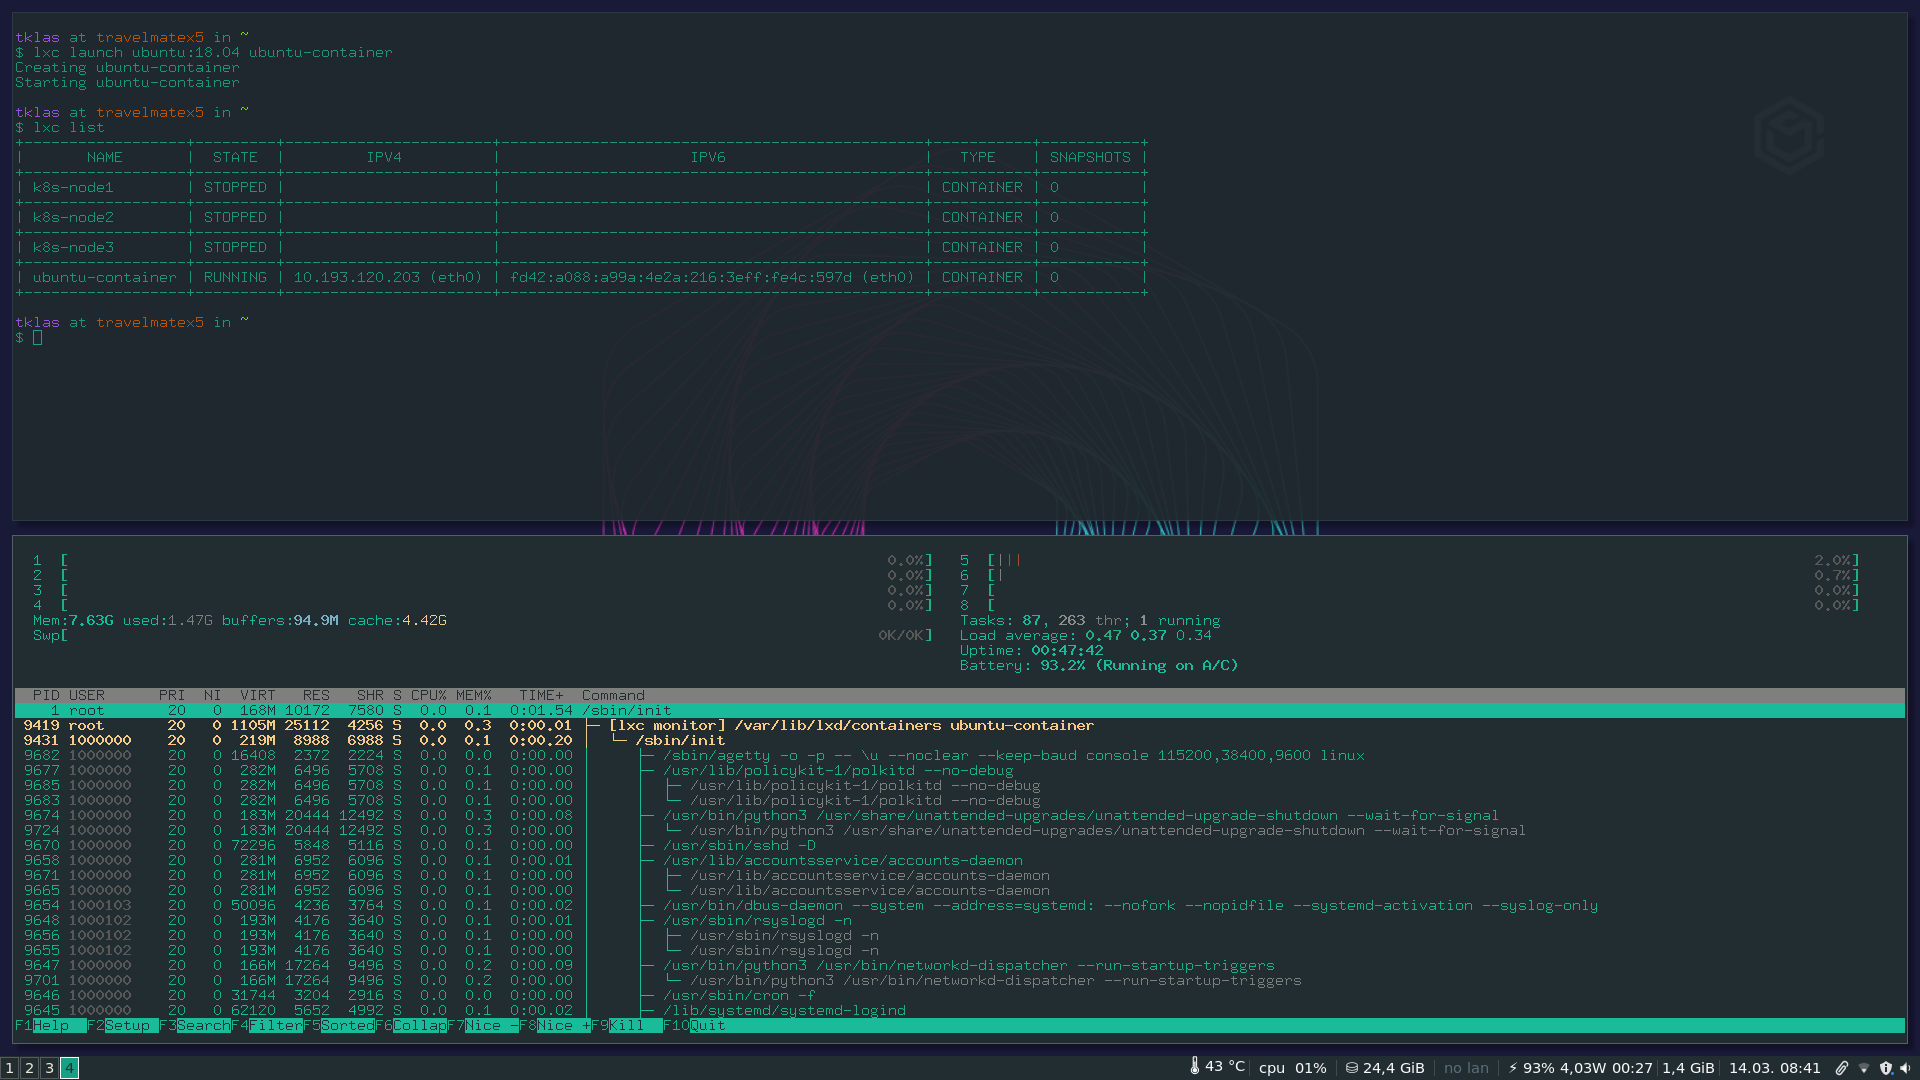
\includegraphics[width=0.95\textwidth, angle=0]{lxc-screen.png}
	\caption[LXC systémové kontejnery]{LXC a jeho procesy.}
	\label{fig:lxc-list}
\end{figure}